%\def\R{$\textsf{R}$}
%\def\S{$\textsf{S}$}

%\renewcommand{\labelitemii}{$\circ$}
\newcommand{\sfa}{a}
\newcommand{\worst}{\mbox{\em worst}}
\newcommand{\best}{\mbox{\em best}}
\newcommand{\regret}{\mbox{\em regret}}
\newcommand{\opt}{\mbox{\em opt}}
\newcommand{\join}{\bowtie}
\newcommand{\lE}{\underline{E}}
\newcommand{\uE}{\overline{E}}
\newcommand{\heads}{{\it heads}}
\newcommand{\tails}{{\it tails}}

\newcommand{\A}{{\cal A}}
\newcommand{\B}{{\cal B}}
\newcommand{\C}{{\cal C}}
\newcommand{\D}{{\cal D}}
\newcommand{\E}{{\cal E}}
\newcommand{\F}{{\cal F}}
\newcommand{\G}{{\cal G}}
%\newcommand{\H}{{\cal H}}
\newcommand{\I}{{\cal I}}
\newcommand{\J}{{\cal J}}
\newcommand{\K}{{\cal K}}
%\newcommand{\L}{{\cal L}}
\newcommand{\M}{{\cal M}}
\newcommand{\N}{{\cal N}}
%\newcommand{\O}{{\cal O}}
\newcommand{\Ocal}{{\cal O}}
\newcommand{\Hcal}{{\cal H}}
\renewcommand{\P}{{\cal P}}
\newcommand{\Q}{{\cal Q}}
\newcommand{\R}{{\cal R}}
%\newcommand{\S}{{\cal S}}
\newcommand{\T}{{\cal T}}
\newcommand{\U}{{\cal U}}
\newcommand{\V}{{\cal V}}
\newcommand{\W}{{\cal W}}
\newcommand{\X}{{\cal X}}
\newcommand{\Y}{{\cal Y}}
\newcommand{\Z}{{\cal Z}}


\newcommand{\IR}{\mathbb{R}}
\newcommand{\dfn}{\begin{definition}}
\newcommand{\edfn}{\end{definition}}
\newcommand{\thm}{\begin{theorem}}
\newcommand{\ethm}{\end{theorem}}
\newcommand{\xam}{\begin{example}}
\newcommand{\exam}{\end{example}}
\newcommand{\inter}{\cap}
\newcommand{\union}{\cup}




\documentclass[t, 8pt, seriff]{beamer}


%\documentclass[a4paper,xcolor=svgnames]{beamer} 
\usepackage[portuguese]{babel}
\usepackage[utf8]{inputenc}
\usepackage{times}
\usepackage{amsmath,amsthm}
\usepackage{amssymb,latexsym}
\usepackage{graphics}
%\usepackage{graphicx}

\usepackage{multimedia}
% \usepackage{movie15}
\usepackage{media9}

\usetheme{default}
%\usetheme{Singapore}
%\usetheme{PaloAlto} 
\usetheme{Boadilla}
% other themes: AnnArbor, Antibes, Bergen, Berkeley, Berlin, Boadilla, boxes, CambridgeUS, Copenhagen, Darmstadt, default, Dresden, Frankfurt, Goettingen,
% Hannover, Ilmenau, JuanLesPins, Luebeck, Madrid, Maloe, Marburg, Montpellier, PaloAlto, Pittsburg, Rochester, Singapore, Szeged, boxes, default

\useoutertheme{infolines}
%\usefonttheme{serif}
% you can also specify font themes: default, professionalfonts, serif, structurebold, structureitalicserif, structuresmallcapsserif

%\definecolor{vermelho}{RGB}{100,30,40}
%\definecolor{vermelholys}{RGB}{132,158,139}
%\definecolor{vermelholyslys}{RGB}{173,190,177}
%\definecolor{vermelholyslyslys}{RGB}{214,223,216}


%\usecolortheme[named=vermelho]{structure}




 



%\documentclass[a4paper,xcolor=svgnames]{beamer} 
%\usepackage[brazil]{babel}
%\usepackage[latin1]{inputenc}
\usepackage{ragged2e}
\usepackage{bm}
\usepackage[T1]{fontenc}
%\usepackage{amsmath,amsthm,amsfonts,amssymb} 
\usepackage{multirow}
%\usetheme{CambridgeUS} 
%\setbeamercolor{normal text}{bg=white}
\usepackage {graphicx,color}

\usepackage{wrapfig} % inserir a figura ao lado do texto
\usepackage[dvips]{epsfig} % inserir figuras de extensao post script (ps)
\usepackage{textcomp}
% \usepackage{undertilde} % colocar o til abaixo do x
\usepackage{multicol} % cor na linha
\usepackage{tabularx}
\usepackage{rotating} %rotacionar figuras e tabelas


\usepackage{ragged2e}
%\justifying


\usepackage{tikz}
\usetikzlibrary{trees}


\newtheorem{lema}{Lema}
\newtheorem{defi}{Definição}
\newtheorem{teo}{Teorema}
\newtheorem{corol}{Corolário}
\newtheorem{prop}{Proposição}


\newtheoremstyle{Exercício}{}{}{\rm}{}{\bf $\bigstar$ }{:}{ }{} %% \scshape para mudar
\theoremstyle{Exercício}
\newtheorem{exer}{Exercício}

\theoremstyle{plain}
\newtheoremstyle{Exemplo}{}{}{\rm}{}{\bf $\rhd$ }{:}{ }{} %% \scshape para mudar
%o tamanho a maiusculo
\theoremstyle{Exemplo}
\newtheorem{exem}{Exemplo}

% 
% \theoremstyle{plain}
% \newtheoremstyle{Nota}{}{}{\rm}{}{\bf\scshape}{:}{ }{}
% \theoremstyle{Nota}
 \newtheorem{nota}{Nota}






%\setlength{\rightskip}{0pt}
%\setlength{\leftskip}{0pt}
%\setlength{\spaceskip}{0pt}
%\setlength{\xspaceskip}{0pt}



\newcommand{\fullpage}[1]{
\begin{frame}
 #1
\end{frame}
}


\setbeamersize{text margin left=3em, text margin right=3em}



\setbeamertemplate{theorems}[numbered]



\definecolor{links}{HTML}{2A1B81}
\hypersetup{colorlinks,linkcolor=,urlcolor=links}


\graphicspath{{./graphics/}} 			% path das figuras (recomendável)

\newcommand{\cor}[1]{ \{{#1}\}}

\title[Probabilidade]{  Probabilidade (PPGECD000000001) \\ \vspace{1cm}Programa de Pós-Graduação em Estatística e Ciência de Dados (PGECD) }
\author[ Raydonal Ospina 
%\textcopyright 
\ ]{
	%Probabilidade\\ 
	Sessão 8 \\
	${}$ \\
	Raydonal Ospina  }

\date[]{}

\institute[UFBA]{Departamento de Estatística\\
	Universidade Federal da Bahia\\
	Salvador/BA}


\usecolortheme[rgb={0,0.6,0.6}]{structure}

%%%%%%%%%%%%%%%%%%%%%%%%%%%%%%%%%%%%%%%%%%%%%%%%%%%%%%%%%%%%%%%%%%%%%%
\begin{document}
% \SweaveOpts{concordance=TRUE}
\begin{frame}
  \titlepage
\end{frame}

%%%%%%%%%%%%%%%%%%%%%%%%%%%%%%%%%%%%%%%%%%%%%%%%%%%%%%%%%%%%%%%%%%%%%%%%%%%%%%%%%%%%%%%%%%%%%%%%%%%%%%%%%%




%=====================================================================
\begin{frame}
	\begin{defi}[Função geradora de momentos de uma variável aleatória]
		\begin{itemize}
			\item Seja $X$ uma variável aleatória discreta, com distribuição de probabilidade $p(x_i) = P(X = x_i)$, $i = 1,2,\ldots$ A {\it função geradora de momentos} da variável $X$ é dada por:
			$$m_X(t) = \sum_{i=0}^\infty  e^{tx_i}p(x_i).$$
			
			\item Seja $X$ uma variável aleatória contínua com função de densidade $f(x)$. A {\it função geradora de momentos} da variável  $X$ é dada por:  
			$$m_X(t) = {\rm E}(e^{tx}) = \int_{-\infty}^{\infty} e^{tx} f(x)dx.$$
		\end{itemize}
	\end{defi}
	%Verifique que $M_X(t)$ gera momentos em torno de a :$E(X - a)^r$, $r = 1,2,\ldots$
	
	%Para $a = 0$, temos os momentos em torno de zero: $EX^r$, $r = 1, 2, \ldots$
	
	%Seja $f(x) = e^x$, expandindo $f(x)$ em série de McLaurin, sendo $a = 0$ temos:
	
	%Para $f(x) = e^x \Longrightarrow f(0) = 1$
	
	%Para $f'(x) = e^x \Longrightarrow f'(0) = 1$
	
	%Para $f''(x) = e^x \Longrightarrow f''(0) = 1$
	
	%$\vdots$                  
	
	%daí:
	
	%$f(x) = 1 + x + \frac{\displaystyle  x^2)}{\displaystyle 2!} +  \frac{\displaystyle x^3}{\displaystyle 3!} + \ldots$
	
	%Analogamente:
	
	%$e^{tX} = 1 + (tX) +\frac{\displaystyle tX^2}{\displaystyle 2!}+  \frac{\displaystyle tX^3}{\displaystyle 3!} + \ldots$
	
	%Para calcularmos o valor esperado temos:
	
	%$M_X(t) = Ee^{tX}= 1 +  (tEX) +\frac{\displaystyle t^2EX^2}{\displaystyle 2!}+  \frac{\displaystyle t^3EX^3}{\displaystyle 3!} + \ldots + \frac{\displaystyle t^nEX^n}{\displaystyle n!}+ \ldots$
	
	%Derivando $M_X(t)$ em relação à t, temos:
	
	%$M'_X(t) = EX + tEX^2 + \frac{\displaystyle t^2EX^3}{\displaystyle 2!} + \ldots + \frac{\displaystyle t^{n - 1}EX^n}{\displaystyle (n - 1)!}+ \ldots$
	
	%Fazendo $t = 0 \Longrightarrow M'_X(t) = EX.$
	
	%Novamente derivando $M_X(t)$ em relação à t, temos:
	
	%$M''_X(t) = EX^2 + tEX^3 + \ldots + \frac{\displaystyle t^{n - 2}EX^n}{\displaystyle (n - 2)!}+ \ldots,$
	
	%e fazendo $t = 0$, temos:
	
	%$M''_X(0)= EX^2$
	
	%Para obtermos $EX^n$, basta calcularmos a derivada {\it n-ésima} de $M_X(t)$ para $t = 0$.
	
	
	
	
	
	
	
	
	
	%%Los momentos de una variable aleatoria $X$ desempe\~{n}an un papel
	%%importante en la estad\'{\i}stica tanto te\'{o}rica como aplicada;
	%%por ello resulta conveniente tener un mecanismo que permita
	%%calcular f\'{a}cilmente, en lo posible, los momentos de la
	%%variable aleatoria. \ Este mecanismo es proporcionado por la
	%%llamada funci\'{o}n generadora de momentos, la cual definiremos a
	%%continuaci\'{o}n.\\
	
	%%\begin{defo}{3.1.4}
	%%La funci\'{o}n generadora de momentos de una variable aleatoria
	%%$X$, denotada por $m_{X}(t)$ se define como sigue:\\
	
	%%\begin{equation*}
	%%m_{X}(t)=E(e^{tX})=\left\{
	%%\begin{array}{c}
	%%\sum_{k}e^{tx_{k}}P(X=x_{k})\;\text{si }X\;\text{es una variable aleatoria
	%%discreta con valores }x_{1},x_{2},\dots \\
	%%\int_{-\infty }^{\infty }e^{tx}f(x)dx\;\;\;\;\;\;\;\;\;\;\text{si }X\;\text{%
	%%es una variable aleatoria con funci\'{o}n de densidad }f.
	%%\end{array}%
	%%\right.\\
	%%\end{equation*}%
	
	O domínio da função $m_{X}(t)$ consiste de todos os $t$ para os quais
	$e^{tX}$ tem valor esperado finito. Se $m_{X}(t)$ é finita em algum intervalo aberto que
	contenha a origem então tem-se que 
	\begin{equation}
	\label{mo1}
	m_{X}(t)={\rm E}(e^{tX})={\rm E}\left(\sum_{n=0}^{\infty }\frac{t^{n}X^{n}}{n!}%
	\right)=\sum_{n=0}^{\infty }\frac{{\rm E}(X^{n})}{n!}t^{n}.
	\end{equation}
\end{frame}
%=====================================================================

%=====================================================================
\begin{frame}
	A expansão em serie de Taylor de $m_{X}(t)$ é 
	\begin{equation}
	\label{mo2}
	m_{X}(t)=\sum_{n=0}^{\infty }\frac{t^{n}}{n!}\frac{d^{n}}{dt^{n}}%
	m_{X}(t)\Bigg\vert _{t=0}.
	\end{equation} 
	Comparando os coeficientes de $t^{n}$ nas equações \eqref{mo1} e \eqref{mo2} temos 
	que os momentos ao redor da origem podem ser obtidos pelas sucessivas derivadas da função geradora de momentos avaliada em $t=0$, isto é,  
	\begin{equation*}
	\mu_n' = {\rm E}{X^{n}}=\frac{d^{n}}{dt^{n}}m_{X}(t)\Big\vert_{t=0}.
	\end{equation*}
	
	\begin{exem}
		Consideremos 
		\begin{center}
			\begin{tabular}{|c|c|c|c|} \hline
				$p(x)$ & 0,3 & 0,5 & 0,2  \\ \hline
				$x$ & 1 & 2 & 3 \\ \hline
			\end{tabular}
		\end{center}
		Logo,  
		$$
		m_{X}(t)={\rm E}(e^{tX})= \sum_x e^{tx} p(x) =0,3e^t+0,5e^{2t}+0,2e^{3t}.
		$$
	\end{exem}
\end{frame}
%=====================================================================

%=====================================================================
\begin{frame}
	\begin{exem}
		Seja $X$ uma v.a. com função de densidade dada por:
		\begin{equation*}
		f_{X}(x)=
		\begin{cases}
		2e^{-2x}& \text{se  }x>0, \\
		0 & \text{    caso contrário}%
		\end{cases}
		\end{equation*}
		e desta forma 
		\begin{equation*}
		m_{X}(t)={\rm E}(e^{tX})=\int_{0}^{\infty }e^{tx}2e^{-2x}dx=\left( 1-\frac{t}{2}%
		\right) ^{-1}\;\text{para }t<\frac{1}{2}.
		\end{equation*}
	\end{exem}
	
	
	\begin{exem}
		Seja $X$ uma variável aleatória com função de probabilidade dada por
		\begin{equation*}
		p(x)=\left\{
		\begin{array}{c}
		e^{-3} \, \frac{3^{x}}{x!}, \;\;\text{se\ }x=0,1,2,... \\
		0\;\;\;\;\;\;\;\;\text{caso contrário.}%
		\end{array}%
		\right.
		\end{equation*}
		Neste caso,
		\begin{equation*}
		m_{X}(t)=\sum_{k=0}^{\infty }e^{tk}e^{-3}\frac{3^{k}}{k!}=\exp
		(3(e^{t}-1)).
		\end{equation*}
	\end{exem}
	
\end{frame}
%=====================================================================


%=====================================================================
\begin{frame}
	\begin{exem}
		Seja $ X $ uma variável aleatória discreta com distribuição binomial com parâmetros $ n $ e $ p $, ou seja, $ X\sim b(n,p) $. Então
		\[
		\begin{aligned}
		m_{X}(t)&={E}\left(e^{tX}\right)=\sum_{x=0}^{n}e^{tx}\left(\begin{array}{c}n\\x\end{array}\right)p^x(1-p)^{n-x} \\
		&=\sum_{x=0}^{n}\left(\begin{array}{c}n\\x\end{array}\right)(e^t p)^x(1-p)^{n-x}=(pe^t+1-p)^{n}.
		\end{aligned}
		\]	
		Podemos encontrar a média e a variância através da função geradora de momentos. Assim
		\[m^\prime_X(t)=\frac{d}{dt}(p e^t+ 1-p)^n=n(pe^t+1-p)^{n-1}pe^t.\]	
		Então como $ {E}(X)=m^\prime_X(0)=n(p+1-p)^{n-1}p=np $. De forma, análoga 
		\[m^{\prime\prime}_X(t)=\frac{d^2}{dt^2}(p e^t+ 1-p)^n=n(n-1)(pe^t+1-p)^{n-2}pe^t pe^t+pe^t n(pe^t+1-p)^{n-1}\]	
		Logo $ {E}\left(X^2\right)=m^{\prime\prime}_X(0)=n(n-1)p^2+ pn $, então obtemos que:
		\[\text{Var}(X)={E}(X^2)-{E}(X)^2=[n(n-1)p^2+pn] -(np)^2=np^2(n-1)+np-n^2p^2=np(1-p).\]	
		
		
		
	\end{exem}
\end{frame}
%=====================================================================


%=====================================================================
\begin{frame}
	\begin{defi}[Quantil]
		
		Seja $p$ um número real qualquer no intervalo unitário $(0, 1)$. Se chama quantil de ordem $p$ de uma variável aleatória $X$
		ou de sua distribuição, um qualquer número $\xi_p$ que cumpre as condições
		$$ P (X \leq \xi_p ) \geq p \qquad \text{e} \qquad P (X \geq \xi_p ) \geq 1 - p. $$
		Quando $p=1/2$ chamamos $\xi_p$ de mediana.
	\end{defi}
	
	
	\begin{exem} 
		Seja $X$ uma variável aleatória discreta tal que $P (X = 1) = 1/2,$ e $P (X = 0) = 1/2.$ Qualquer número no intervalo [0, 1] é uma mediana de $X.$
	\end{exem}
	O anterior exemplo nos permite verificar que os quantis não são necessariamente únicos e desta forma motivamos o uso de uma definição mais rigorosa para o quantil.
	
	\begin{defi}[Função quantil]
		Para $0<p<1,$ a função 
		\begin{equation}
		\label{fquantil}
		\xi_p=F^{-1}(p)=\inf\{x |F(x)\geq p\}
		\end{equation}
		é chamada de {\bf função quantil} (ou inversa da função de distribuição) e 
		o valor $\xi_p$ é o quantil de ordem $p.$ 
		Em particular, $\xi_{\frac{1}{2}}=  F^{-1}(1/2)$ é chamado da \textbf{mediana} de $F$. 
	\end{defi}
	
	
\end{frame}
%=====================================================================

%=====================================================================
\begin{frame}
	
	\begin{figure}[!htb]
		\begin{center}
			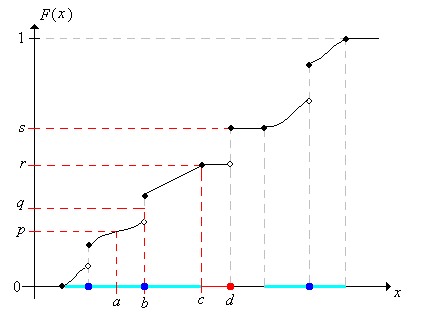
\includegraphics[scale=0.3]{quantile.png} 
			\caption{\label{figquant} Representação gráfica da função quantil.}
		\end{center}
	\end{figure}
	
	\begin{figure}[!htb]
		\begin{center}
			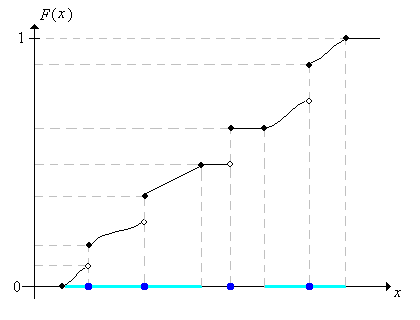
\includegraphics[scale=0.3]{CDFMixed.png} 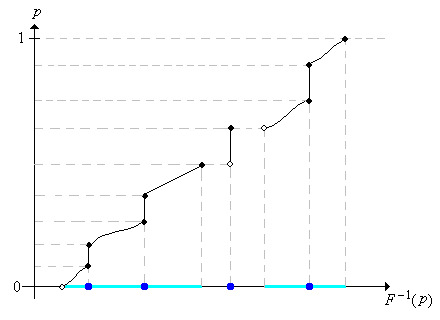
\includegraphics[scale=0.3]{QuantileFunction.png} 
			\caption{\label{figquant} Representação gráfica da função quantil.}
		\end{center}
	\end{figure}
	
\end{frame}
%=====================================================================



%=====================================================================
\begin{frame}
	\begin{exem}
		Consideremos $X$ uma variável aleatória com função de densidade e distribuição acumulada  dada por:
		$$
		f(x)=
		\begin{cases}
		2{\rm e}^{-2x} & \text{para} \ x>0, \\
		0 & \text{caso contrário},
		\end{cases}
		\quad 
		F(x)=
		\begin{cases}
		1-{\rm e}^{-2x} & \text{para} \ x>0 \\
		0 & \text{caso contrário}.
		\end{cases}
		$$
		Logo, 
		$$\xi_p=F^{-1}(p) =-2 \ln(1-p), \ 0<p<1$$ é a sua função quantil. Aqui o valor da mediana é $\xi_{\frac{1}{2}}=\ln(4).$ 
	\end{exem}
	
	\begin{teo}{(Transformação integral da probabilidade).}  
		Seja $X$ uma v.a. contínua com distribuição $F$ então, $Y=F(x) \sim U(0,1),$ isto é, a função de densidade de $Y$ é 
		$$
		f(y)=
		\begin{cases}
		1 & \text{para} \ 0<y<1, \\
		0 & \text{caso contrário}.
		\end{cases}
		$$
	\end{teo}
	\begin{nota}[Uso: Geração de variáveis aleatórias]
		Se queremos gerar uma variável aleatória $ X $ com $ F_X(x) = \mathbb{P}(X\leq x) $ para todo $ x $. então  geramos uma variável aleatória $ U $ uniforme em $ [0,1] $, isto é, $ U\sim U[0,1] $ e então, a variável aleatória $ X = F_X^{-1}(U).$
	\end{nota}
\end{frame}
%=====================================================================




\begin{frame}

\begin{block}{Distribuição condicional de $X$ dado $A$}
	
	Seja $X$ uma variável aleatória no espaço de probabilidade
	$(\Omega,\A,P)$, e seja $A$ um evento aleatório tal que $P(A)>0$.
	Usando o conceito de probabilidade condicional, podemos definir a
	distribuição condicional de $X$ dado o evento $A$ por
	$$P(X\in B|A)=\frac{P([X\in B]\cap A)}{P(A)},$$
	para $B$ boreliano. Pode-se verificar facilmente que isto define uma
	probabilidade nos borelianos verificando-se os axiomas. Podemos
	interpretar a distribuição condicional de $X$ dado $A$ como a nova
	distribuição que se atribui a $X$ quando sabe-se da ocorrência do
	evento $A$. A função de distribuição associada à distribuição
	condicional é chamada função distribuição condicional de $X$ dado
	$A$:
	$$F_X(x|A)=P(X\leq x|A).$$
	A esperança condicional de $X$ dado $A$ é a esperança da
	distribuição condicional, definida por
	$$E(X|A)=\int xdF_X(x|A),$$
	se esta esperança existe.
	
\end{block}
\end{frame}

\begin{frame}

\begin{block}{}


Agora suponhamos que os eventos aleatórios $A_1,A_2,\ldots$ formem
uma partição (finita ou enumerável) de $\Omega$. Pelo Teorema da
Probabilidade Total, temos
$$P(X\in B)=\sum_n P(A_n)P(X\in B|A_n),\forall B\in \B,$$
e
\begin{eqnarray}
& & F_X(x)=P(X\leq x)=\sum_n P(A_n)P(X\leq x|A_n) \nonumber \\
& & =\sum_n P(A_n)F_X(x|A_n), \forall x \nonumber,
\end{eqnarray}

e se a esperança de $X$ existe,
\begin{eqnarray}
& & EX=\int xdF_X(x)=\int x d(\sum_n P(A_n)F_X(x|A_n)) \nonumber \\
& & =\sum_n P(A_n)\int x dF_X(x|A_n)=\sum_n P(A_n)E(X|A_n)\nonumber.
\end{eqnarray}

\end{block}
Em outras palavras, a distribuição de $X$ (resp., função de
distribuição, esperança de $X$) é uma média ponderada da
distribuição condicional (resp., função de distribuição condicional,
esperança condicional de $X$) dado $A_n$, onde os pesos são as
probabilidades dos membros $A_n$ da partição.
\end{frame}


\begin{frame}

\begin{block}{Distribuição condicional de $X$ dado $Y$ Discreto}


Consideremos agora o caso em que a partição do espaço amostral é
gerada por uma variável aleatória discreta. Para tanto, seja $Y$ uma
variável aleatória discreta em $(\Omega,\A, P)$, tomando somente os
valores $y_1,y_2,\ldots$. Então, os eventos $A_n=[Y=y_n]$ formam uma
partição de $\Omega$. Neste caso, a distribuição
$$P(X\in B|Y=y_n)=P(X\in B|A_n),$$
para $B$ boreliano, é chamada de distribuição condicional de $X$
dado que $Y=y_n$, e valem as fórmulas
\begin{eqnarray}
& & P(X\in B)=\sum_n P(Y=y_n)P(X\in B|Y=y_n),
\nonumber \\
& & F_X(x)=\sum_n P(Y=y_n)F_X(x|Y=y_n), \nonumber \\
& & EX=\sum_n P(Y=y_n)E(X|Y=y_n), \nonumber
\end{eqnarray}
onde vale a última fórmula se $EX$ existe; em particular, se $X$ é
integrável.

\end{block}
\end{frame}

\begin{frame}
\begin{block}{}


Notemos que para $B$ fixo, $P(X\in B|Y=y_n)$ é função de $y_n$,
digamos $g(y_n)$. Se definirmos $g(y)=P(X\in B|Y=y)$ arbitrariamente
para $y\notin \{y_n:n\geq 1\}$, por exemplo, $g(y)=P(X\in B)$, então
teremos
\begin{eqnarray}
& & P(X\in B)=\int P(X\in B|Y=y)dF_Y(y)
\nonumber\\
& & =\int g(y)dF_Y(y),
\nonumber \end{eqnarray}
pelas propriedades da integral de Lebesgue no caso de $Y$ discreto.
As outras fórmulas possuem interpretações análogas, logo teremos
\begin{eqnarray}
& & P(X\in B)=\int P(X\in B|Y=y)dF_Y(y),
\nonumber \\
& & F_X(x)=\int F_X(x|Y=y)dF_Y(y), \nonumber \\
& & EX=\int E(X|Y=y)dF_Y(y). \nonumber
\end{eqnarray}
\end{block}
Essas fórmulas valem também no caso geral, como veremos adiante.
Salientamos que a esperança precisa existir para que a última
fórmula valha. De fato, quando $X$ for integrável,
$\varphi(y)=E(X|Y=y)$ será finito.
\end{frame}

\begin{frame}
\begin{block}{}
Nesse caso, a variável aleatória
$\varphi(Y)$ será chamada de esperança condicional de $X$ dada $Y$ e
será indicada por $\varphi(Y)=E(X|Y)$. Notemos que $E(X|Y=y)$ é um
valor particular da variável aleatória $E(X|Y)$: é o valor quando
$Y=y$. Portanto, a última fórmula pode ser reescrita assim
$$EX=E\varphi(Y)=E(E(X|Y)).$$
Em outras palavras, a esperança de $X$ é igual à esperança da
esperança condicional de $X$ dada $Y$.
\end{block}

\begin{exem}
Consideremos o seguinte experimento em que participam dois
jogadores, I e II. Suponhamos que o jogador I lance uma moeda
honesta $n$ vezes, obtendo $k$ caras, onde $0\leq k\leq n$, e que
depois disso o jogador II lance a mesma moeda $k$ vezes. Seja $X$ o
número de caras obtidas pelo jogador II. Qual a esperança de $X$
supondo independência de todos os lançamentos?

Seja $Y$ o número de caras nos $n$ lançamentos do jogador I. Decorre
das condições do experimento que $Y \thicksim b(n,\frac{1}{2})$ e
que $X|Y=k \thicksim b(k,\frac{1}{2})$. Por isso, a esperança
condicional de $X$ dado que $Y=k$ é a esperança da distribuição
$b(k,\frac{1}{2})$: $E(X|Y=k)=\frac{k}{2}$, ou seja,
$E(X|Y)=\frac{Y}{2}$. Utilizando a fórmula, temos
$$EX=E(E(X|Y))=E(\frac{Y}{2})=\frac{n}{4}.$$
\end{exem}

\end{frame}

\begin{frame}
\begin{exem}
Consideremos outro jogo que conta com a participação de dois jogadores I e II. Neste jogo, o jogador I vai fazer uma sequência de lançamentos independentes de uma moeda que tem probabilidade $p$ de dar cara, onde $0<p<1$. Antes do jogador I começar, o jogador II observa uma variável aleatória $N$ tendo distribuição $Poisson(\lambda)$, onde $\lambda>0$. Supomos que $N$ seja independente da sequência de lançamentos do jogador I. Se o jogador II observar $N=n$, ele vai parar o jogador I depois de ter feito $n$ lançamentos (se $N=0$, o jogador II não permite nenhum lançamento). Se $S$ for o número de caras observadas até o jogador I parar, qual é a esperança de S?

\bigskip
{\bf Solução:} Como a sequência de lançamentos é independente de $N$, a distribuição condicional de $S$ dado que $N=n$ é $binomial(n,p)$. Portanto, $E(S|N=n)=np$, ou seja, $E(S|N)=Np$. Logo,
$$ES=E(Np)=pEN=p\lambda.$$
\end{exem}

\bigskip
Agora, queremos definir a distribuição condicional de
$X$ dado que $Y=y$ para todo $y\in R$ e todo par de variáveis
aleatórias $X$ e $Y$ definidas no mesmo espaço de probabilidade
$(\Omega,\A,P)$.  Anteriormente definimos a distribuição
condicional dado que $Y=y$ quando $P(Y=y)>0$; portanto nosso
problema agora é como definir distribuição condicional quando
$P(Y=y)=0$. 

\end{frame}

\begin{frame}
\begin{block}{Distribuição condicional de $X$ dado $Y$ Qualquer}

No caso discreto essa definição era arbitrária, pois o
conjunto $B_0=\{y_n:n=1,2,\ldots\}^c$ também tinha probabilidade
zero. Mas é evidente que essa solução não serve no caso geral, já
que no caso continuo $P(Y=y)=0$ para todo $y\in R$.

\end{block}

\begin{block}{}


Para termos uma intuição sobre a definição formal da distribuição condicional no caso geral,
consideremos novamente o caso discreto. Pelas fórmulas obtidas na
seção anterior a distribuição (resp., função de distribuição,
esperança) de $X$ é determinada pela distribuição $Y$ e a
distribuição (resp., função de distribuição, esperança) condicional
de $X$ dada $Y$. De fato, o Teorema da Probabilidade Total nos dá um
resultado muito mais forte: a distribuição conjunta de $X$ e $Y$ é
determinada pela distribuição de $Y$ e a distribuição condicional de
$X$ dada $Y$. Para ver isto, basta notar que para todo $x$ e $y$,
\begin{eqnarray}
& & F_{X,Y}(x,y)=P(X\leq x, Y\leq y)=\sum_{n:y_n\leq y}P(X\leq
x,Y=y_n) \nonumber \\
& & =\sum_{n:y_n\leq y}P(Y=y_n)P(X\leq x|Y=y_n) =\sum_{n:y_n\leq
y}P(Y=y_n)F_X(x|Y=y_n) \nonumber \\
& & =\int_{-\infty}^{y}F_X(x|Y=t)dF_Y(t). \nonumber
\end{eqnarray}


\end{block}
\end{frame}

\begin{frame}
\begin{block}{}
Vemos então que no caso discreto a função de distribuição conjunta é
uma espécie de composta da função de distribuição marginal de $Y$
com a função de distribuição condicional de $X$ dada $Y$. E pode-se
provar que para todo par de variáveis aleatórias $X$ e $Y$,
definidas no mesmo espaço de probabilidade, existe uma, e somente
uma, família de funções de distribuição condicional satisfazendo a
condição acima. Isto justifica a seguinte definição formal para a distribuição condicional
de $X$ dada $Y$:
\end{block}
\begin{defi}
	\label{def_form1} Sejam $X$ e $Y$ variáveis aleatórias definidas no
	mesmo espaço de probabilidade $(\Omega, \A, P)$. Uma função $P(X\in
	B|Y=y)$, definida para $B$ boreliano e $y\in R$, será chamada uma
	distribuição condicional (regular) para $X$ dada $Y$ se
	\begin{enumerate}
		\item[(i)] para todo $y\in R$ fixo, $P(X\in B|Y=y)$ define uma
		probabilidade na $\sigma$-álgebra de Borel; e
		
		\item[(ii)] para todo $B$ boreliano fixo, $P(X\in B|Y=y)$ é função
		mensurável de $y$ e para todo $(x,y)\in R^2$,
		$$\int_{-\infty}^{y}F_X(x|Y=t)dF_Y(t)=F_{X,Y}(x,y).$$
	\end{enumerate}
\end{defi}
\end{frame}

\begin{frame}
O próximo teorema prova que esta definição determina uma única distribuição condicional quase certamente.

\begin{teo}
Sejam $X$ e $Y$ variáveis aleatórias em $(\Omega,\A,P)$. Então
existe uma distribuição condicional regular para $X$ dada $Y$.
Existe apenas uma, no sentido de que duas distribuições condicionais
são iguais quase certamente: se $P_1(X\in B|Y=y)$ e $P_2(X\in
B|Y=y)$ são ambas distribuições condicionais para $X$ dada $Y$,
então existe um boreliano $B_0$ tal que $P(Y\in B_0)=1$ e $P_1(X\in
B|Y=y)=P_2(X\in B|Y=y)$, para todo $B$ boreliano e $y\in B_0$.
\end{teo}


Existe uma outra alternativa para se calcular a distribuição
condicional de $X$ dada $Y$ que utiliza uma aproximação da definição do caso
discreto. Para tanto, seja $I$ um intervalo pequeno de comprimento
$\Delta y$ e que contém o ponto $y$. Tomemos como aproximação para a
probabilidade condicional de $X$ pertencer a $B$ dado que $Y=y$, a
probabilidade condicional do mesmo evento dado que $Y\in I$, ou
seja,
\begin{eqnarray}
& & P(X\in B|Y=y)\approx P(X\in B|Y\in I)=\frac{P(X\in B,Y\in I)}{P(Y\in I)}.\nonumber
\end{eqnarray}

Se $P(X\in B|Y=y)$ converge para um limite quando $\Delta y\rightarrow 0$, chama-se o limite de $P(X\in B|Y=y)$. Se $P(Y\in I)=0$ para algum intervalo $I$ ao redor de $y$, então pode-se definir a probabilidade condicional arbitrariamente, por exemplo, pode-se fazer $P(X\in B|Y=y)=P(X\in B)$. O seguinte teorema prova que esta maneira alternativa de calcular a distribuição condicional
de $X$ dado $Y$ quase sempre coincide com a Definição~\ref{def_form1}.
\end{frame}

\begin{frame}
\begin{theorem}
Para cada $B$ boreliano fixo, o limite na definição 4.2 existe quase
certamente, i.e., $P(Y\in \{y:\mbox{ limite existe em }y\})=1$. Além
disso, para cada $B$ fixo, o limite é igual a $P(X\in B|Y=y)$ como
definido na Definição~\ref{def_form1}, quase certamente, ou seja, o conjunto dos
$y$'s para os quais o limite converge para $P(X\in B|Y=y)$ conforme a Definição~\ref{def_form1} tem probabilidade 1.
\end{theorem}

Tanto a Definição~\ref{def_form1} quanto o método da aproximação por limites não são úteis para
encontrar a distribuição condicional. Para tanto deve-se tentar
adivinhar um candidato. Consideremos alguns casos simples em que a solução vem de imediato:

\begin{block}{Caso I: $Y$ discreta}

Considere a solução que obtivemos quando analisamos o caso discreto. Portanto, se $Y$ assume os valores $y_1,y_2,\ldots$ tais que
$P(Y=y_n)>0$, então
$$P(X\in B|Y=y_n)=\frac{P(X\in B,Y=y_n)}{P(Y=y_n)}, \forall B\in\B,$$
e $P(X\in B|Y=y)=P(X\in B)$ se $P(Y=y)=0$. Note que esta distribuição satisfaz as duas condições da Definição~\ref{def_form1} e portanto é uma distribuição condicional de acordo com a definição do caso geral.

\end{block}
\end{frame}

\begin{frame}
\begin{block}{Caso II: $X$ e $Y$ independentes}

Intuitivamente, a distribuição condicional de $X$ dado que $Y=y$ não deveria depender de $y$. Portanto, nosso candidato é:
$$P(X\in B|Y=y)=P(X\in B), \forall B\in \B,\forall y\in\IR.$$
Portanto, a primeira condição da Definição~\ref{def_form1} é satisfeita e nosso candidato para $F_X(x|Y=y)$ é $F_X(x)$, logo
\begin{eqnarray}
& & \int_{-\infty}^{y}F_X(x)dF_Y(t)=F_X(x)\int_{-\infty}^{y}dF_Y(t)=F_X(x)F_Y(y)=F_{X,Y}(x,y),\nonumber
\end{eqnarray}
ou seja, a segunda condição da definição também é satisfeita.
\end{block}

\begin{block}{Caso III: $X$ e $Y$ possuem densidade conjunta $f(x,y)$}

Neste caso nosso candidato será
$$f(x|y)=\frac{f(x,y)}{f(y)}, x\in R,$$
se $f(y)>0$, e $f(x|y)=f(x)$ se $f(y)=0$. Esta função é chamada de
densidade condicional de $X$ dado que $Y=y$. Note que $f(x|y)$
preserva as chances relativas e realmente é uma densidade. 

\end{block}
\end{frame}

\begin{frame}
\begin{block}{}
	Agora,
	vamos mostrar que ela satisfaz a Definição~\ref{def_form1}. Parte
	(i), segue do fato que $f(x|y)$ é uma densidade de probabilidade e
	portanto $P(X\in B|Y=y)=\int_{X\in B} f(x|y)dx$ é uma probabilidade
	para todo boreliano $B$. Para verificar (ii), note que a função de
	distribuição condicional é $F_X(x|Y=t)=\int_{-\infty}^{x}f(s|t)ds$.
	Logo
	\begin{eqnarray}
	& & \int_{-\infty}^{y}(\int_{-\infty}^{x}f(s|t)ds)dF_Y(t)\nonumber\\
	& & =
	\int_{-\infty}^{y}(\int_{-\infty}^{x}\frac{f(s,t)}{f_Y(t)}ds)f_Y(t)dt=\int_{-\infty}^{y} \int_{-\infty}^{x} f(s,t)ds dt=F_{X,Y}(x,y).\nonumber
	\end{eqnarray}
	\end{block}

\begin{block}{Caso IV: $X$ discreta e $Y$ com densidade $f_Y$}

De acordo com a definição de distribuição condicional, ela deve satisfazer neste caso:
$$\int_{-\infty}^{y}P(X=x_i|Y=t)f_Y(t)dt=P(X=x_i,Y\leq y).$$
Note que se definirmos
\begin{eqnarray}
& & P(X=x_i|Y=t)=\frac{1}{f_Y(t)}\frac{\partial P(X=x_i,Y\leq t)}{\partial t}\nonumber \\
& &=\frac{1}{f_Y(t)}\frac{\partial P(Y\leq t|X=x_i)P(X=x_i)}{\partial t}  = \frac{P(X=x_i)}{f_Y(t)}f_{Y|X}(t|x_i), \nonumber
\end{eqnarray}
obtemos o resultado desejado.

\end{block}
\end{frame}

\begin{frame}
\begin{block}{Princípios}

Em casos mais complexos, no processo de escolha da distribuição condicional, ajuda observar os seguintes
princípios:

\begin{itemize}
\item {\bf Princípio da preservação das chances relativas.} Este
princípio diz que condicionalmente, dada a ocorrência de um evento
$A$, os resultados possíveis (ou seja, $w\in A$) mantêm as mesmas
chances relativas que tinham antes da realização do experimento.

\item {\bf Princípio da substituição.} Este princípio diz que
condicionalmente, dado que $Y=y$, a variável aleatória $Y$ pode ser
substituída pelo valor $y$ sempre que $Y$ aparecer em uma
probabilidade (ou esperança) condicional. Mais geralmente, diz que
para obter a distribuição condicional de $\varphi(X,Y)$ dado que
$Y=y$, basta substituir $Y$ pelo valor $y$.
\end{itemize}
\end{block}

\begin{exem}
Seja $X$ uma variável aleatória simétrica em torno de zero, de modo que $P(X\leq x)=P(X\geq -x), \forall x\in \IR$. Qual a distribuição condicional de $X$ dado $|X|$?
\end{exem}


\end{frame}

\begin{frame}
\begin{block}{Solução}

Utilizando o princípio da preservação das chances relativas e a simetria da variável $X$, temos que nosso candidato para distribuição condicional deve ser:
$P(X=y||X|=y)=P(X=-y||X|=y)=1/2$ se $y>0$ e $P(X=0||X|=0)=1$. Como
\begin{eqnarray}
& & \int_{0}^{y}P(X\leq x||X|=t)dF_{|X|}(t)
\nonumber\\
& & =\left \{
\begin{array}{cc}
\int_{0}^{y} 0 dF_{|X|}(t) & \mbox{, se $x<-y$} \\
\int_{0}^{|x|^-} 0 dF_{|X|}(t)+\int_{|x|^-}^{y} \frac{1}{2} dF_{|X|}(t) & \mbox{, se $-y\leq x<0$}\\
\int_{0^-}^{x} 1 dF_{|X|}(t)+\int_{x}^{y} \frac{1}{2} dF_{|X|}(t)  &  \mbox{, se $0\leq x<y$}\\
\int_{0^-}^{y} 1 dF_{|X|}(t) & \mbox{, se $x\geq y\geq 0$}
\end{array}
\right.
\nonumber\\
& & =\left \{
\begin{array}{cc}
0 & \mbox{, se $x<-y$} \\
1/2(F_{|X|}(y)-F_{|X|}(|x|^-)) & \mbox{, se $-y\leq x<0$} \\
1/2(F_{|X|}(y)+F_{|X|}(x))  &  \mbox{, se $0\leq x<y$}\\
F_{|X|}(y) & \mbox{, se $x\geq y\geq 0$}
\end{array}
\right.
\nonumber\\
& & =\left \{
\begin{array}{cc}
0 & \mbox{, se $x<-y$} \\
F_X(x)-F_X(-y^-) & \mbox{, se $-y\leq x<0$}\\
F_X(x)-F_X(-y^-)  &  \mbox{, se $0\leq x<y$}\\
F_{|X|}(y) & \mbox{, se $x\geq y\geq 0$}
\end{array}
\right.\nonumber
\end{eqnarray}
Mas esta última expressão é igual a $F_{X,|X|}(x,y)$. Portanto, nosso candidato satisfaz a definição de distribuição condicional.
%\end{example}

\end{block}
\end{frame}

\begin{frame}

\begin{exem}
Se $f_{Y|X}(y|x)=|x+1|e^{-|x+1|y}U(y)$ e $X\sim Binomial(2,1/2)$, qual a densidade de $Y$? Dado que $Y=y$, qual a distribuição de $X$ para $y>0$?
\end{exem}


\begin{block}{Solução}

\begin{eqnarray}
& & f_Y(y)=\sum_{i=0}^{2}|i+1|e^{-|i+1|y}U(y)\binom{2}{i}(1/2)^2 \nonumber \\
& & =\frac{1}{4}U(y)(e^{-y}+4e^{-2y}+3e^{-3y}) \nonumber
\end{eqnarray}

Utilizando o resultado do Caso IV acima temos que
\begin{eqnarray}
& & P(X=i|Y=y)=\frac{P(X=i)}{f_Y(y)}f_{Y|X}(t|i) \nonumber \\
& & =\frac{\binom{2}{i}|i+1|e^{-|i+1|y}}{(e^{-y}+4e^{-2y}+3e^{-3y})}, i=0,1,2. \nonumber
\end{eqnarray}
%\end{example}

\end{block}
\end{frame}

\begin{frame}{Esperança Condicional}

\begin{defi}
Sejam $X$ e $Y$ variáveis aleatórias em $(\Omega,\A,P)$. A esperança
condicional de $X$ dado que $Y=y$, é a esperança da distribuição
condicional de $X$ dado que $Y=y$, se esta esperança existir. Ou
seja,
$$E(X|Y=y)=\int x dF_X(x|Y=y).$$
\end{defi}

Pode-se provar que:

\begin{teo}
	Se $X$ é integrável, então $E(X|Y=y)$ existe e é finita quase
	certamente, i.e., existe um boreliano $B_0$ tal que $P(Y\in B_0)=1$
	e $E(X|Y=y)$ é finita para todo $y\in B_0$.
\end{teo}

Se definirmos $\varphi(y)=E(X|Y=y)$, a variável aleatória
$\varphi(Y)=E(X|Y)$ chama-se esperança condicional de $X$ dada $Y$.
A esperança condicional, sendo a esperança da distribuição
condicional, possui todas as propriedades da esperança ordinária
(por exemplo, linearidade, desigualdade de Jensen, convergência
monótona, convergência dominada), mais a propriedade importante de
que $E(E(X|Y))=EX$, ou seja
$$EX=\int E(X|Y=y)dF_Y(y).$$

\end{frame}

\begin{frame}
\begin{block}{}
Já demonstramos esta equação no caso discreto, vamos verificá-las
quando $X$ e $Y$ têm densidade conjunta $f(x,y)$:
\begin{eqnarray}
& & E(X|Y=y)=\int xdF_X(x|Y=y)=\int_{-\infty}^{\infty}xf(x|y)dx\nonumber\\
& & =\int_{-\infty}^{\infty}x\frac{f(x,y)}{f_Y(y)}dx,\nonumber
\end{eqnarray}
se $f_{Y}(y)>0$. Logo, quando $X$ é integrável,
\begin{eqnarray}
& & E(E(X|Y))=\int
E(X|Y=y)dF_Y(y)\nonumber\\
& & =\int_{-\infty}^{\infty}(\int_{-\infty}^{\infty}x\frac{f(x,y)}{f_Y(y)}dx
f_Y(y)dy) \nonumber \\
& & =\int_{-\infty}^{\infty}\int_{-\infty}^{\infty}x f(x,y)dx
dy=\int_{-\infty}^{\infty}(\int_{-\infty}^{\infty} f(x,y)dy) x dx
\nonumber \\
& & =\int_{-\infty}^{\infty}x f_X(x)dx = EX. \nonumber
\end{eqnarray}
\end{block}
\end{frame}

\begin{frame}
\begin{block}{}


Como $A=[I_A=1]$, temos
\begin{eqnarray}
& & E(I_A|Y=y)=1\cdot P(I_A=1|Y=y)\nonumber\\
& & +0\cdot P(I_A=0|Y=y) \nonumber
\\
& & =P(I_A=1|Y=y)=P(A|Y=y). \nonumber
\end{eqnarray}
De fato, como $I_A$ é integrável, nós temos
$$P(A)=E(I_A)=E(E(I_A|Y))=E(P(A|Y)),$$
ou seja, a probabilidade de um evento é a esperança de sua
probabilidade condicional dada $Y$, para qualquer $Y$.


\end{block}
\end{frame}

\begin{frame}
\begin{block}{Propriedades}


A seguir enumeramos algumas propriedades da esperança condicional, que são generalizações de propriedades da esperança incondicional.

\begin{enumerate}
\item[EC1.] $E(E(X|Y))=EX$.

\item[EC2.] Se $X=c$, para alguma constante $c$, então $E(X|Y)=c$.

\item[EC3.] Se $X_1\leq X_2$, então $E(X_1|Y)\leq E(X_2|Y)$.

\item[EC4.] $E(aX_1+bX_2|Y)=aE(X_1|Y)+bE(X_2|Y)$.

\item[EC5.] Seja $\phi$ uma função convexa. Então, $\phi(E(X|Y))\leq E(\phi(X)|Y)$.

\item[EC6.] Se $X_n\geq 0$ e $X_n\uparrow X$, então $E(X_n|Y)\uparrow E(X|Y)$.

\item[EC7.] Se $X_n\rightarrow X$ e se existe $X_0$ integrável tal que $|X_n|\leq X_0$, então $\lim_n E(X_n|Y)=E(X|Y)$.

\item[EC8.] Se $\phi(X,Y)$ é integrável, então
\begin{eqnarray}
& & E(\phi(X,Y)|Y=y)=E(\phi(X,y)|Y=y)\nonumber\\
& & =\int\phi(x,y)dF_X(x|Y=y).\nonumber
\end{eqnarray}
\end{enumerate}

\end{block}
\end{frame}

\begin{frame}{Outros Momentos Condicionais}


Assim como no caso incondicional podemos definir momentos condicionais de ordem mais elevada de maneira análoga. O $k$-ésimo momento de $X$ dado $Y$ é dado por $E(X^k|Y)$. E o $k$-ésimo momento central é dado por $E((X-E(X|Y))^k|Y)$. Em particular, o segundo momento central é conhecido como variância condicional de $X$ dado $Y$ e pode ser reescrito como:
\begin{eqnarray}
& & Var(X|Y)=E((X-E(X|Y))^2|Y)\nonumber\\
& & =E(X^2|Y)-(E(X|Y))^2.
\nonumber
\end{eqnarray}

\begin{exem}
Sejam $X$ e $Y$ variáveis aleatórias independentes e identicamente distribuídas, com $X\sim U[0,1]$, e sejam $U=\min(X,Y)$ e $V=\max(X,Y)$. Encontre $E(U|V)$.
\end{exem}

\end{frame}

\begin{frame}
\begin{block}{Solução}


\begin{eqnarray}
& & F_{U,V}(x,y)=P(U\leq x,V\leq y)=P(V\leq y)-P(U>x,V\leq y) \nonumber \\
& & =\left \{\begin{array}{cc}
P(X\leq y,Y\leq y)-P(x<X\leq y,x<Y\leq y) & \mbox{, se $x<y$} \\
P(X\leq y,Y\leq y) & \mbox{, se $x\geq y$.}
\end{array}
\right. \nonumber
\end{eqnarray}

Portanto, como $X$ e $Y$ são independentes, temos
$$F_{U,V}(x,y)=\left \{\begin{array}{cc}
0 & \mbox{, se $x\leq 0$ ou $y\leq 0$}\\
y^2-(y-x)^2 & \mbox{, se $0<x<y<1$} \\
y^2 & \mbox{, se $0<y\leq x$ e $y<1$}\\
1-(1-x)^2 & \mbox{, se $y\geq 1$ e $0<x<1$}\\
1 & \mbox{, se $y\geq 1$ e $x\geq 1$.}
\end{array}
\right.$$

Logo,
$$f_{U,V}(x,y)=\frac{\partial^2 F_{U,V}(x,y)}{\partial x\partial y}=\left \{\begin{array}{cc}
2 & \mbox{, se $0<x<y<1$} \\
0 & \mbox{, caso contrário.}
\end{array}
\right.$$
Como $f_V(y)=\int f_{U,V}(x,y)dx=\int_{0}^{y}2dx=2y$, se $0<y<1$, e $f_V(y)=0$ caso contrário, temos que
$$f_{U|V}(x|y)=\frac{f_{U,V}(x,y)}{f_{V}(y)}=\left \{\begin{array}{cc}
\frac{1}{y} & \mbox{, se $0<x<y<1$} \\
0 & \mbox{, caso contrário.}
\end{array}
\right.$$

\end{block}
\end{frame}

\begin{frame}
\begin{block}{}


Então,
$$E(U|V=y)=\int xf_{U|V}(x|y)dx=\int_{0}^{y}\frac{x}{y}dx=\frac{y}{2},$$
se $0<y<1$, e $E(U|V=y)=0$, caso contrário.
Portanto, $$E(U|V)=\left \{\begin{array}{cc}
\frac{V}{2} & \mbox{, se $0<V<1$} \\
0 & \mbox{, caso contrário.}
\end{array}
\right.$$
\end{block}

\begin{exem}
Sejam $X_1,\ldots,X_n$ independentes, identicamente distribuídas e integráveis, e seja $S=X_1+\cdots+X_n$. Demonstre que $E(X_i|S)=\frac{S}{n}$, para $i=1,2,\ldots,n$.
\end{exem}

\end{frame}

\begin{frame}
\begin{block}{Solução}


Note que os vetores $$(X_1,\ldots,X_n)\mbox{ e }(X_i,X_2,\ldots,X_{i-1},X_1,X_{i+1},\ldots,X_n)$$ têm a mesma distribuição. Isto implica que $(X_1,S)$ e $(X_i,S)$ possuem a mesma distribuição. Como a distribuição conjunta determina a distribuição condicional, temos que $X_1$ e $X_i$ têm a mesma distribuição condicional dado que $S=s$, e consequentemente tem a mesma esperança condicional dado $S=s$. Portanto,
$$E(X_1|S=s)=E(X_2|S=s)=\ldots=E(X_n|S=s).$$
Utilizando a linearidade da esperança, temos
\begin{eqnarray}
& & nE(X_i|S=s)=\sum_{i=1}^{n}E(X_i|S=s) \nonumber \\
& & =E(\sum_{i=1}^{n}X_i|S=s)=E(S|S=s)=s. \nonumber
\end{eqnarray}
Então, podemos concluir que $E(X_i|S=s)=\frac{s}{n}$, ou seja, $E(X_i|S)=\frac{S}{n}$.


\end{block}
\end{frame}

\begin{frame}
\begin{exem}
Sejam $X$ e $Y$ duas variáveis aleatórias. Calculemos a distribuição
de $Z=X+Y$. Temos
\begin{eqnarray}
& & P(X+Y\leq z)=E(P(X+Y\leq z|Y))\nonumber\\
& & =\int P(X+Y\leq z|Y=y)dF_Y(y)
\nonumber \\
& & \int P(X\leq z-y|Y=y)dF_Y(y)\nonumber\\
& & =\int F_X(z-y|Y=y)dF_Y(y). \nonumber
\end{eqnarray}
Se $X$ e $Y$ são independentes, então $F_X(z-y|Y=y)=F_X(z-y)$ e
temos
\begin{eqnarray}
& & F_Z(z)=P(X+Y\leq z)=\int F_X(z-y)dF_Y(y).\nonumber
\end{eqnarray}
Esta distribuição é a convolução das distribuições de $X$ e $Y$.
\end{exem}
\end{frame}




\end{document}

